\documentclass{beamer}
\usepackage{amsmath}
\usepackage{amssymb}
\usepackage{bm}
\usepackage{graphicx}
\usepackage{epstopdf}
\usepackage[c]{mcode}
\usepackage{listings}
\usepackage{multicol}
\usepackage{multimedia}
\usepackage{sansmathaccent}
\pdfmapfile{+sansmathaccent.map}
\newcommand{\mbf}{\mathbf}
 \newcommand{\bq}{\begin{equation}}
 \newcommand{\eq}{\end{equation}}
 \newcommand\scalemath[2]{\scalebox{#1}{\mbox{\ensuremath{\displaystyle #2}}}}

\usetheme{CambridgeUS}
\title{A 2D Godunov Solver for the Euler Equations on Non-Cartesian Domains}
\subtitle{Numerical Solutions of Wave Equation - MATH 6890}

\author{Michael Hennessey \inst{1}}
\institute[RPI]
{
\inst{1}
Department of Applied Mathematics\\
Rensselaer Polytechnic Institute}

\date{December 5, 2016}

\subject{2D Non-Cartesian Euler}

\begin{document}

\begin{frame}
\titlepage
\end{frame}

\begin{frame}{Outline}
\begin{multicols}{2}
\tableofcontents
\end{multicols}
\end{frame}

\section{Preliminaries}
\subsection{Motivation}
\begin{frame}{Motivation}
\begin{itemize}
\item{
	Gas Dynamics
	}
\item{
	Atmospheric Science
	}
\item{
Reactive Euler Equations and Detonations
}
\end{itemize}
\end{frame}

\begin{frame}{Governing Equations}
\begin{equation}
\mbf{U}_t+\mbf{F}_x+\mbf{G}_y=0,
\end{equation}
where
\begin{equation}
\mbf{U}=\left[\begin{array}{c}\rho\\ \rho u\\ \rho v\\ E\end{array}\right],\;\;
\mbf{F}=\left[\begin{array}{c}\rho u \\ \rho u^2+p \\ \rho u v\\ u(E+p)\end{array}\right],\;\;
\mbf{G}=\left[\begin{array}{c}\rho v\\ \rho uv\\ \rho v^2+p\\ v(E+p)\end{array}\right].
\end{equation}
Equation of State: $E=\frac{1}{2}\rho(u^2+v^2)+\rho e.$\\
Ideal Gas:
\bq PV=nRT\;\;\implies e=\frac{p}{\rho(\gamma-1)}.\eq
\end{frame}

\subsection{Model Problems}
\begin{frame}{Model Problems}
\begin{itemize}
\item 1D Equations on a Line

\item 2D Equations on a Box
\begin{itemize}
\item Closed Box

\item Open Box

\item Free Space (Rectangular Domain)
\end{itemize}
\item 2D Equations on an Annulus 
\item 2D Equations on a Quarter Circle
\end{itemize}
\end{frame}
\section{Solution Methods}
\subsection{Riemann Problems}
\begin{frame}{Solution Methods for the Riemann Problem}
In order to compute fluxes $(\mbf{F}, \mbf{G})$ across interfaces, we need to have some solution method to the Riemann problem
\bq \begin{split}
&\mbf{U}_t+\mbf{F}_x+\mbf{G}_y=0,\\
&\mbf{U}(x,y,0)=\left\{\begin{array}{cc}\mbf{U}_L,&x<0\\ \mbf{U}_R,&x>0\end{array}\right., \text{or} \left\{\begin{array}{cc}\mbf{U}_B,&y<0\\ \mbf{U}_T,&y>0\end{array}\right..
\end{split} \eq
\begin{itemize}
\item Exact Solution
\begin{itemize}
\item Pros: High Accuracy, Easy to Extend to Higher Orders of Accuracy, Preserves Exact Wave-Form
\item Cons: Heavy Computation Cost - Adaptive Iterative Solver
\end{itemize}
\item Approximate Solution (HLLC)
\begin{itemize}
\item Pros: OK Accuracy, Low Computation Cost
\item Cons: Does not Preserve Exact Wave Form
\end{itemize}
\end{itemize}
\end{frame}


\subsection{Exact Riemann Solution}
\begin{frame}{Exact Riemann Solution}
\begin{itemize}
\item Shocks and the Hugoniot Locus
\begin{itemize}
\item The Rankine-Hugoniot Conditions
\bq 
\mbf{F}(\tilde{\mbf{U}})-\mbf{F}(\hat{\mbf{U}})=S(\tilde{\mbf{U}}-\hat{\mbf{U}})
\eq
\end{itemize}

\item Rarefactions and Integral Curves
\begin{itemize}
\item The Generalized Riemann Invariants
\bq \frac{dp}{d\rho}=a^2=\frac{\gamma p}{\rho},\;\;\; ad\rho+\rho du=0.\eq
\end{itemize}

\item Form of the Exact Solution
\end{itemize}
\begin{figure}[f]
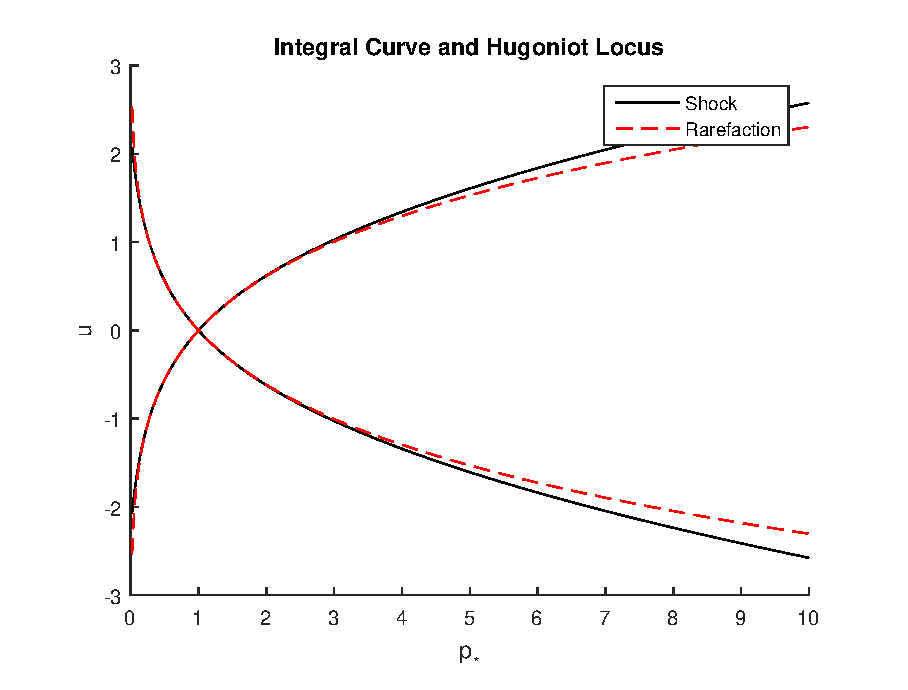
\includegraphics[width=1.5in]{hugoniot1}
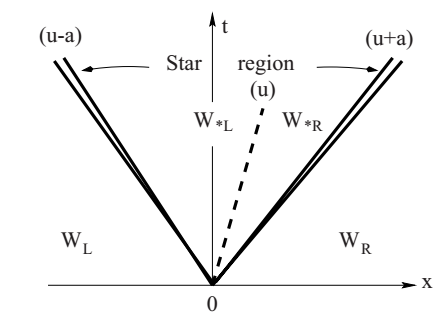
\includegraphics[width=1.5in]{riemannsoln}
\end{figure}

\end{frame}


\begin{frame}{The Adaptive Iterative Solver}
\begin{itemize}

\item Parameterization
\begin{itemize}
\item $p_*$ - Easy, Only for Nice EoS
\item $\rho_{*R},\rho_{*L}$ - Hard, Works well for Hard EoS
\end{itemize}
\item Initial Guess
\begin{itemize}
\item Linearized Guess
\item Double Rarefaction Guess
\item Double Shock Guess
\end{itemize}

\item The Newton Problem
\bq p^{n+1}=p^n-\frac{F_L(p^n)+F_R(p^n)+u_R-u_L}{F'_L(p^n)+F'_R(p^n)}\eq
Where $F_k$ is either an integral curve or a Hugoniot locus.\\
Solution is Adaptive - changes $F_k$ each iteration based on wave-form!
\end{itemize}
\end{frame}

\subsection{HLLC Riemann Solution}
\begin{frame}{Approximate Riemann Solution}
\begin{itemize}
\item Many approximate solutions - Roe, HLL, PVRS, TRRS,TSRS, ANRS,...
\item HLLC Solver - Harten, Lax, van Leer + Contact
\begin{itemize}
\item Direct Approximation of Intercell Flux
\item Complete Solver - All Characteristic Fields Accounted For
\item Algorithmically Determine Wave Speeds $\rightarrow$ Closed-Form Expression for Flux
\end{itemize}
\end{itemize}
\end{frame}

\subsection{A Comparison of the Exact and HLLC Solvers}
\begin{frame}{A Comparison of the Exact and HLLC Solvers}
We will solve the Riemann Problem using each Solver
$$\mbf{U}_t+\mbf{F}_x+\mbf{G}_y=0$$
$$\mbf{U}(x,y,0)=\left\{\begin{array}{cc}\mbf{U}_L,&x<0\\ \mbf{U}_R,&x>0\end{array}\right.$$

\begin{itemize}
\item Double Shock
\bq \mbf{U}_L=\left[\begin{array}{c}5.99924\\ 19.5975\\ 0\\ 460.894\end{array}\right],\;\; \mbf{U}_R=\left[\begin{array}{c}5.99242\\ -6.19633 \\ 0\\ 46.0950\end{array}\right].\eq

\item Double Rarefaction
\bq \mbf{U}_L=\left[\begin{array}{c}1\\ -2\\ -3\\ 0.4\end{array}\right],\;\; \mbf{U}_R=\left[\begin{array}{c}1\\ 2 \\ 3\\ 0.4\end{array}\right].\eq
\end{itemize}
\end{frame}

\begin{frame}{A Comparison of the Exact and HLLC Solvers}
$$\mbf{U}_t+\mbf{F}_x+\mbf{G}_y=0$$
$$\mbf{U}(x,y,0)=\left\{\begin{array}{cc}\mbf{U}_L,&x<0\\ \mbf{U}_R,&x>0\end{array}\right.$$

\begin{itemize}
\item Left Rarefaction, Right Shock
\bq \mbf{U}_L=\left[\begin{array}{c}1\\ 0\\ 0\\ 1000\end{array}\right],\;\; \mbf{U}_R=\left[\begin{array}{c}1\\ 0 \\2\\ 0.01\end{array}\right].\eq
\item Left Shock, Right Rarefaction
\bq \mbf{U}_L=\left[\begin{array}{c}1\\0\\1\\1\end{array}\right],\;\; \mbf{U}_R=\left[\begin{array}{c}1.5\\ 0 \\ 0\\2\end{array}\right].\eq
\end{itemize}
\end{frame}


\begin{frame}{Double Shock}
\begin{figure}[ht]
\centering
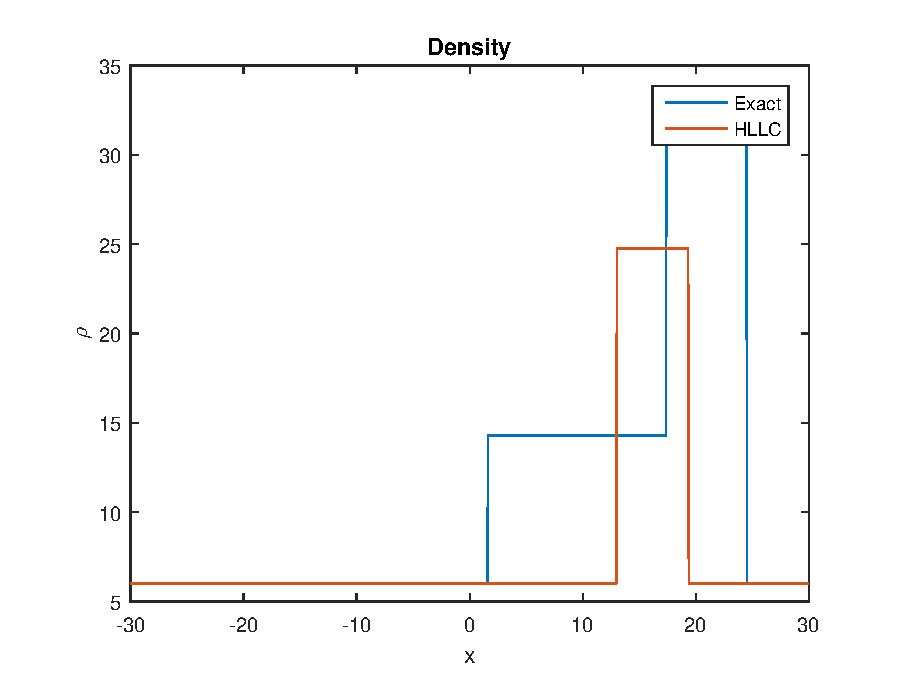
\includegraphics[width=1.8in]{dubShockDen}
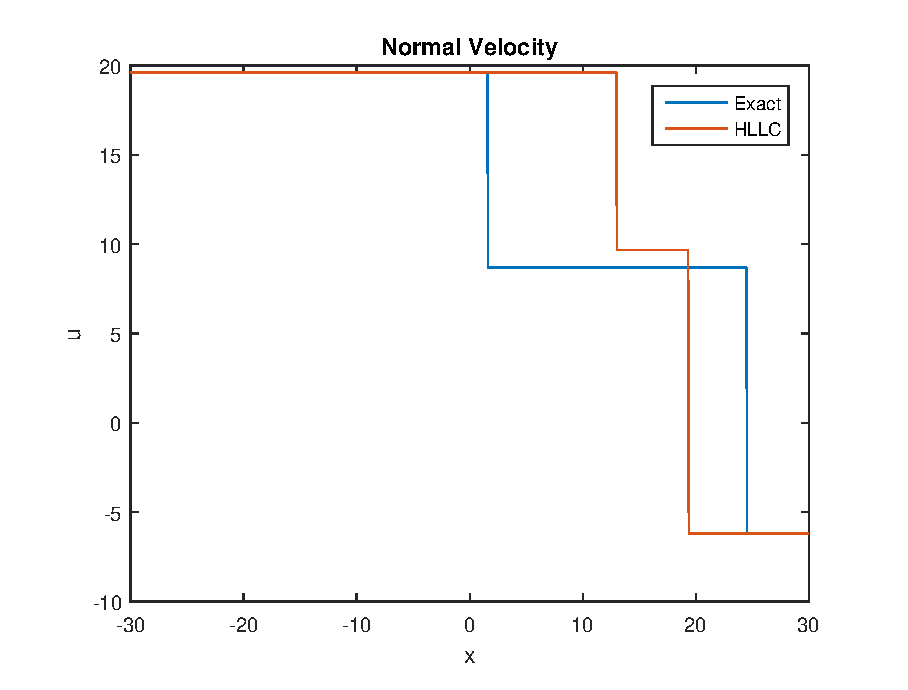
\includegraphics[width=1.8in]{dubShockU}\\
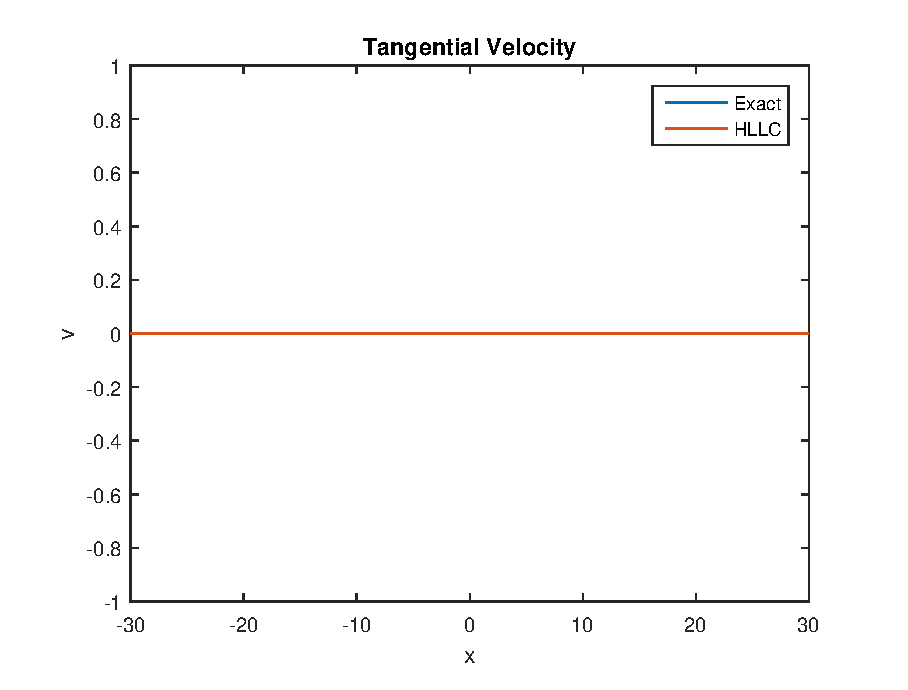
\includegraphics[width=1.8in]{dubShockV}
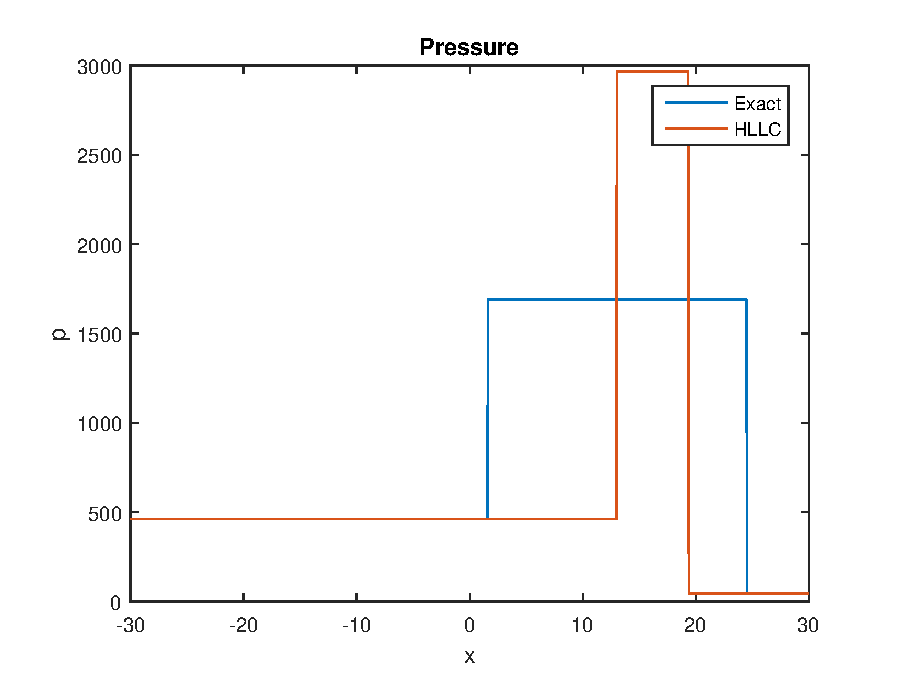
\includegraphics[width=1.8in]{dubShockP}
\end{figure}
\end{frame}

\begin{frame}{Double Rarefaction}
\begin{figure}[ht]
\centering
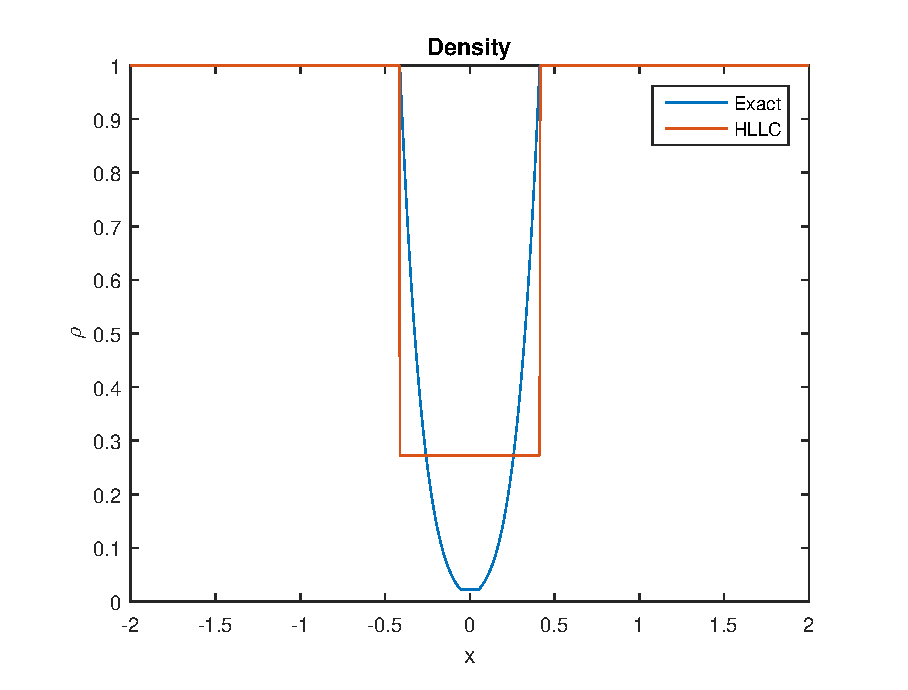
\includegraphics[width=1.8in]{dubRareDen}
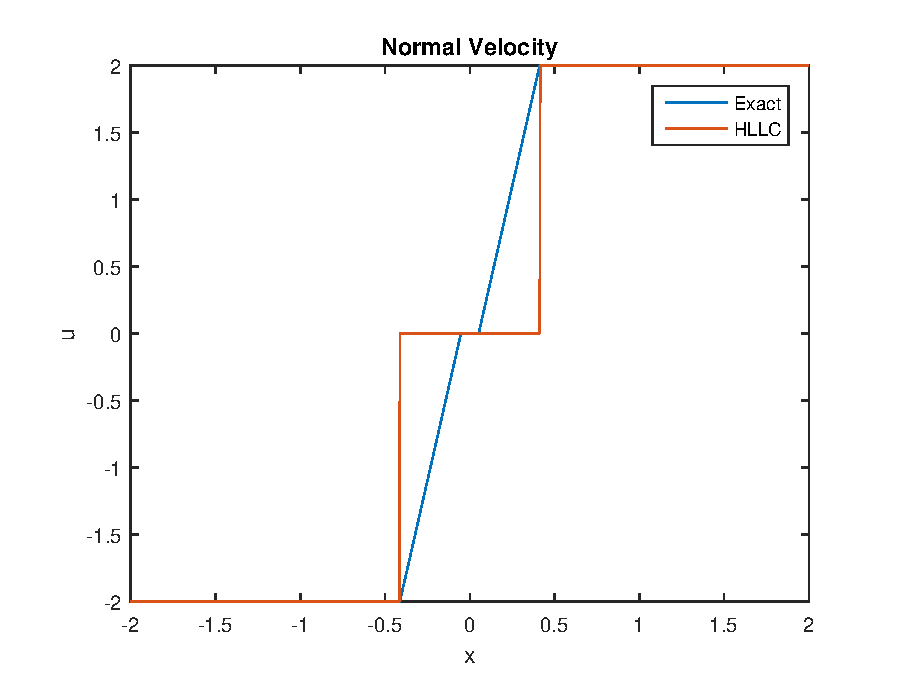
\includegraphics[width=1.8in]{dubRareU}\\
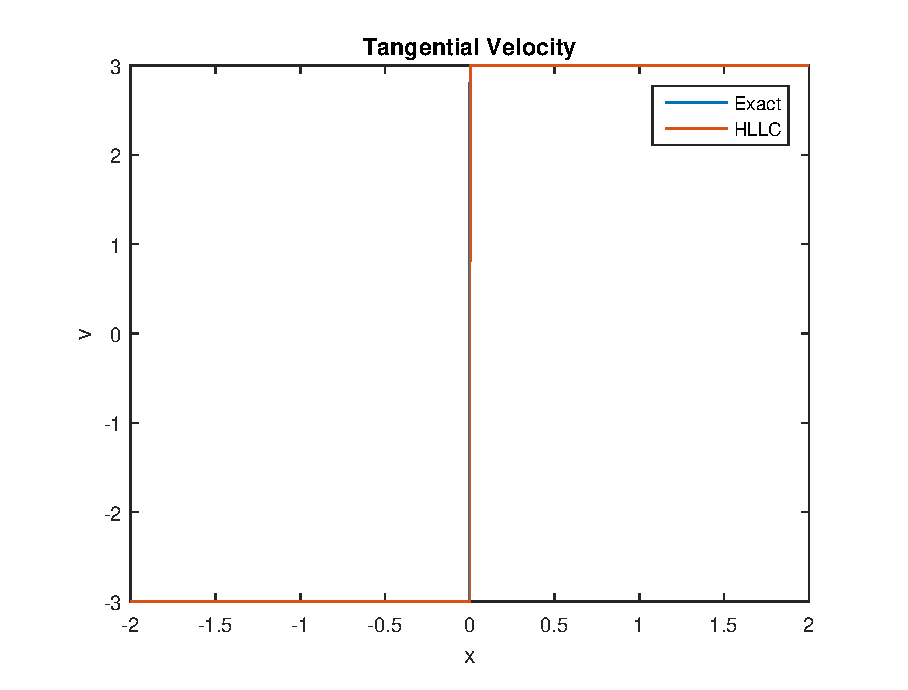
\includegraphics[width=1.8in]{dubRareV}
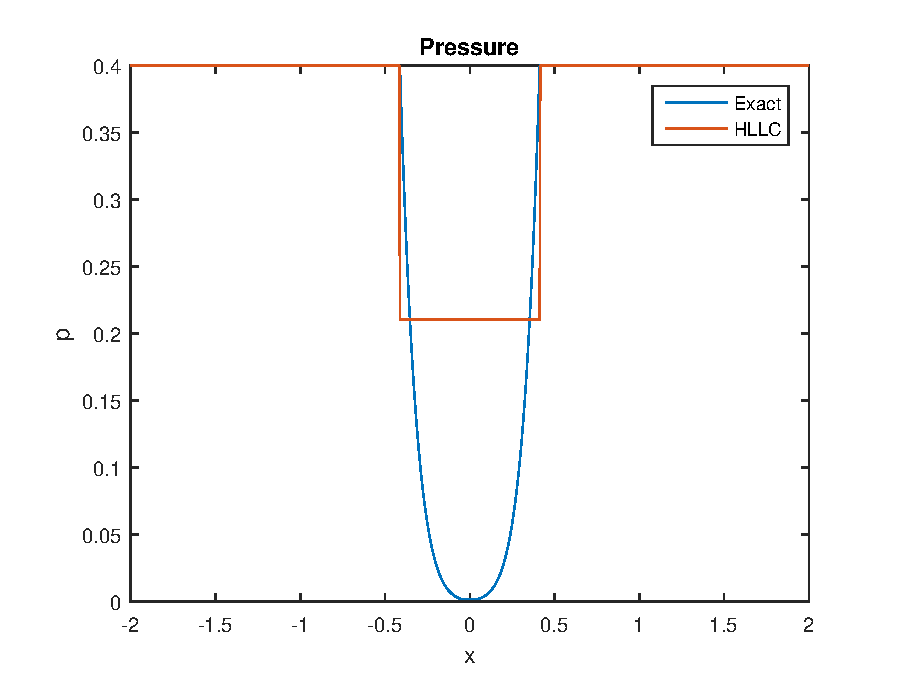
\includegraphics[width=1.8in]{dubRareP}
\end{figure}
\end{frame}

\begin{frame}{Left Rarefaction, Right Shock}
\begin{figure}[ht]
\centering
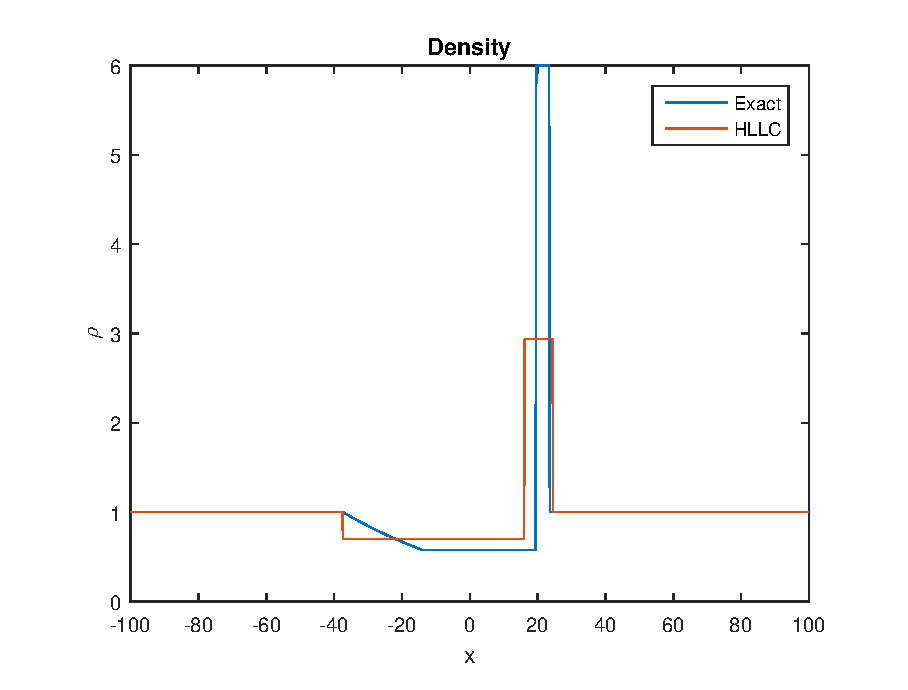
\includegraphics[width=1.8in]{lRareDen}
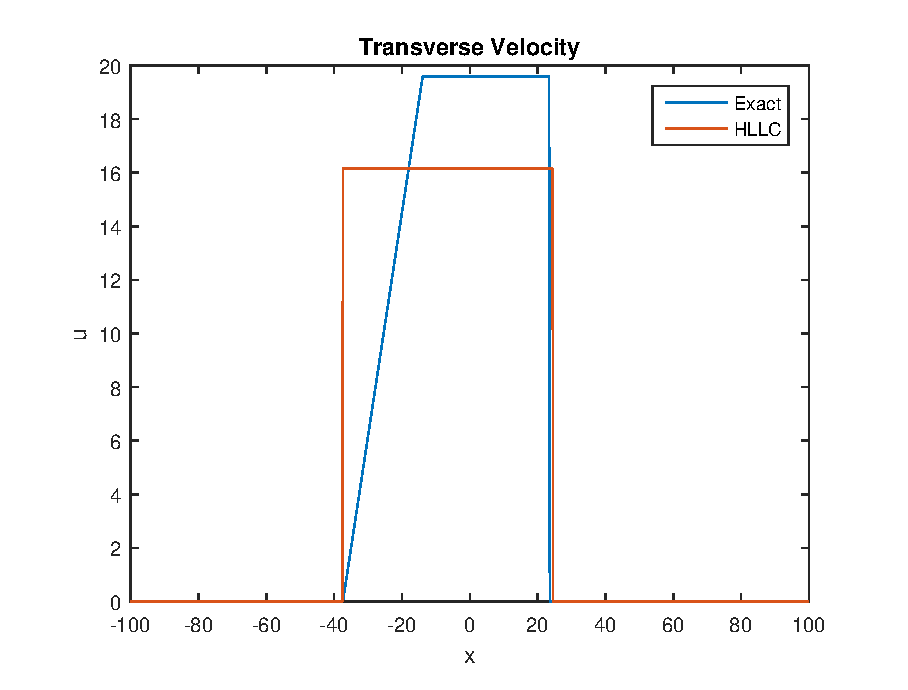
\includegraphics[width=1.8in]{lRareU}\\
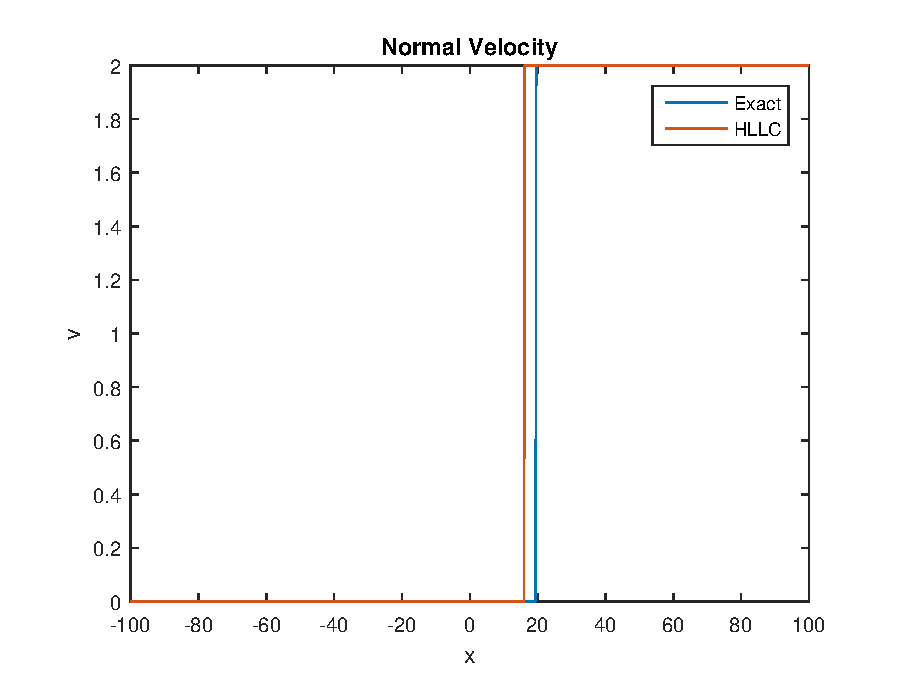
\includegraphics[width=1.8in]{lRareV}
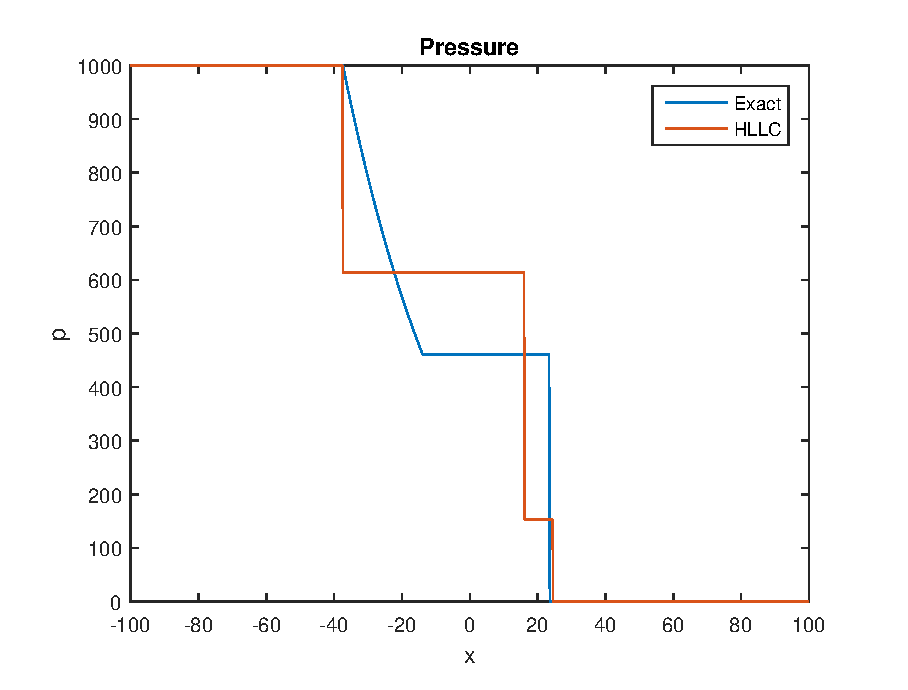
\includegraphics[width=1.8in]{lRareP}
\end{figure}
\end{frame}

\begin{frame}{Left Shock, Right Rarefaction}
\begin{figure}[ht]
\centering
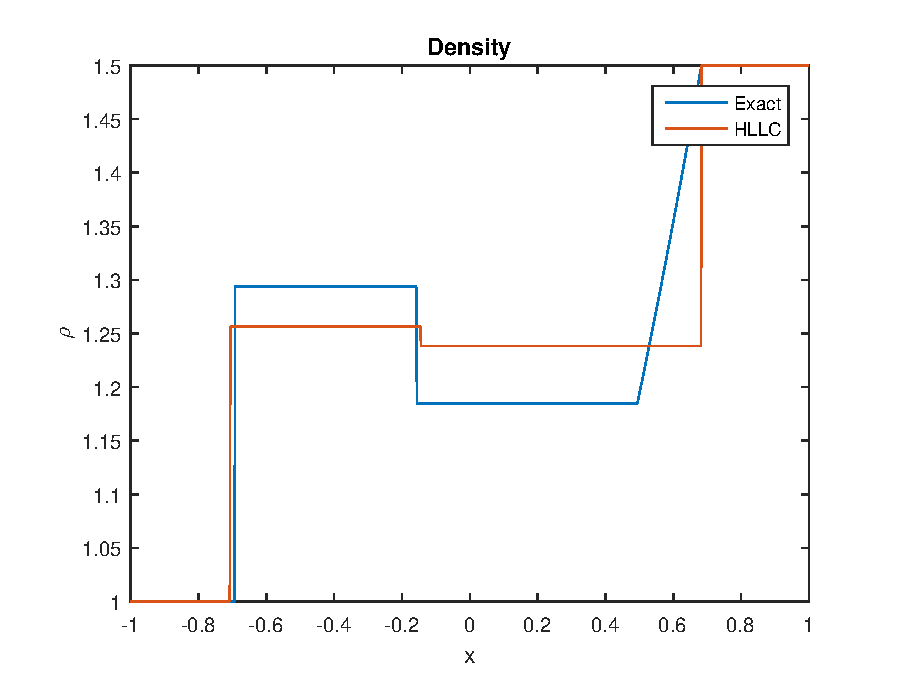
\includegraphics[width=1.8in]{lShockDen}
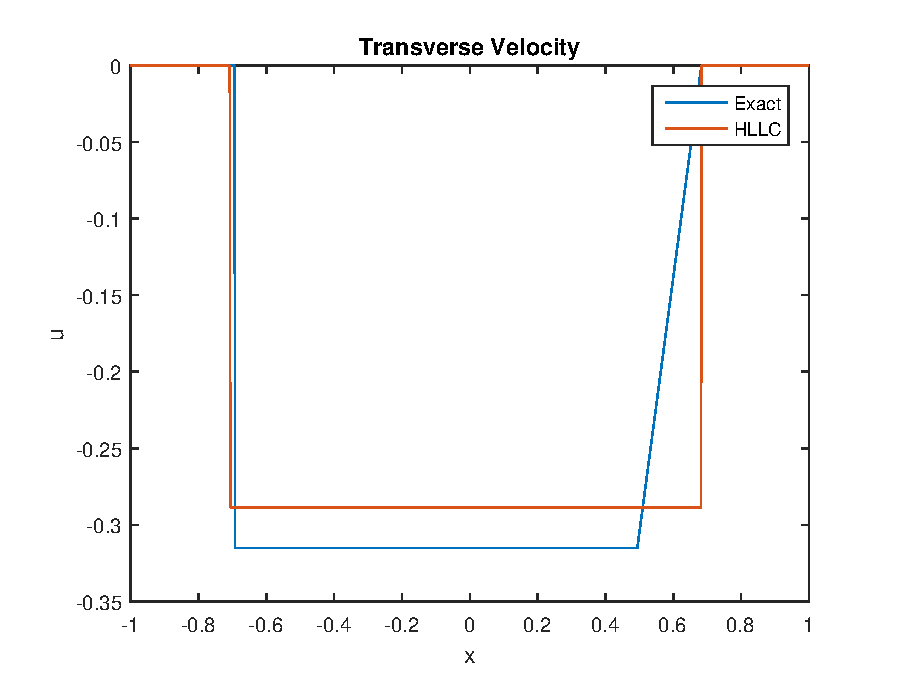
\includegraphics[width=1.8in]{lShockU}\\
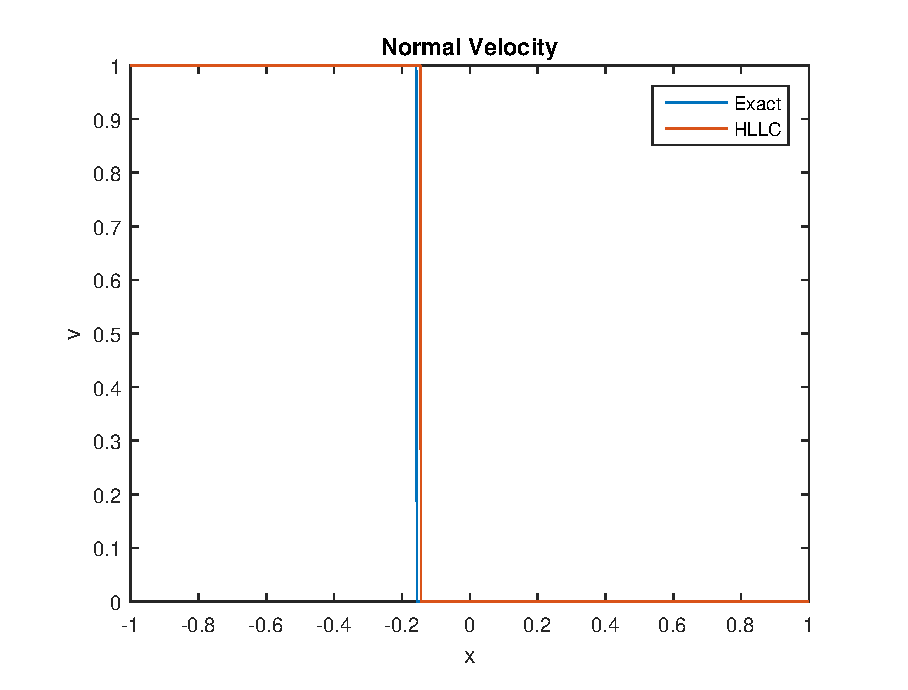
\includegraphics[width=1.8in]{lShockV}
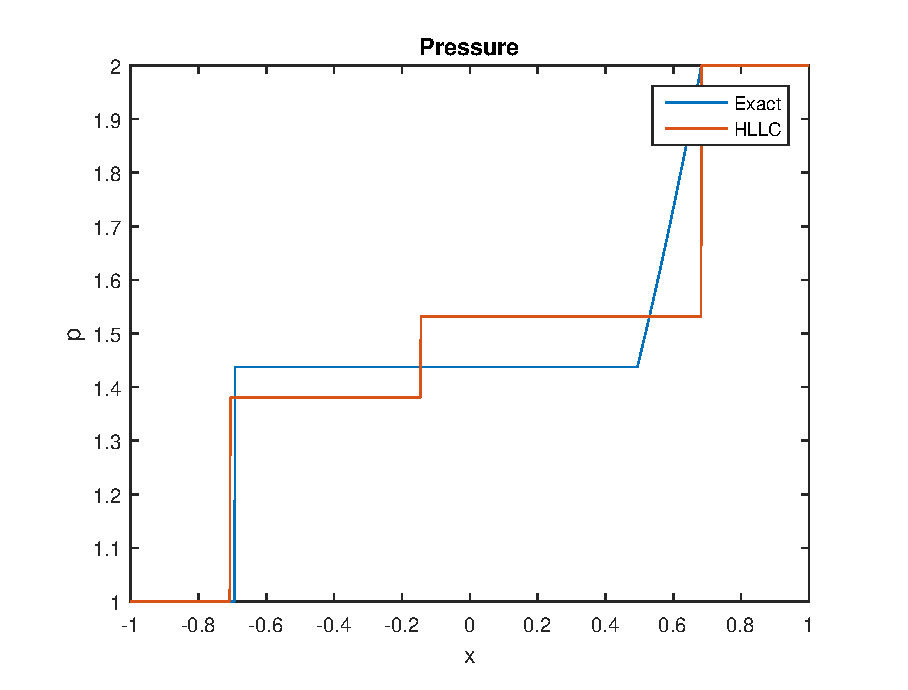
\includegraphics[width=1.8in]{lShockP}
\end{figure}
\end{frame}

\section{The Numerical Method}
\subsection{Discretization}
\begin{frame}{Discretization}
Finite Volume Method:\\
Cell Average: $\mbf{U}_{j,k}^n=\frac{1}{\Delta x \Delta y}\int_{y_{k-1/2}}^{y_{k+1/2}}\int_{x_{j-1/2}}^{x_{j+1/2}}\mbf{U}(\xi,\eta,t_n)d\xi d\eta$\\
Integrate Conservation Law:
\bq \scalemath{.8}{\frac{1}{\Delta x \Delta y}\int_{t_n}^{t_{n+1}}\int_{y_{k-1/2}}^{y_{k+1/2}}\int_{x_{j-1/2}}^{x_{j+1/2}}[\mbf{U}_t(\xi,\eta,\tau)+\mbf{F}_x(\mbf{U}(\xi,\eta,\tau))+\mbf{G}_y(\mbf{U}(\xi,\eta,\tau))]d\xi d\eta d\tau=0}\eq
Resultant Discretization:
\bq 
\scalemath{.9}{
\begin{split}
\mbf{U}_{j,k}^{n+1}=\mbf{U}_{j,k}^n&-\frac{\Delta t}{\Delta x}[\mbf{F}(\mbf{U}(x_{j+1/2},y_k,t_{n+1/2}))-\mbf{F}(\mbf{U}(x_{j-1/2},y_k,t_{n+1/2}))]\\
&-\frac{\Delta t}{\Delta y}[\mbf{G}(\mbf{U}(x_j,y_{k+1/2},t_{n+1/2}))-\mbf{G}(\mbf{U}(x_j,y_{k-1/2},t_{n+1/2}))]\end{split}}\eq

\end{frame}


\subsection{Boundary Conditions}
\begin{frame}{Boundary Conditions}
\begin{itemize}
\item Reflective Boundary
\bq \rho_{M+1,k}^n=\rho_{M,k}^n,\;\; u_{M+1,k}^n=-u_{M,k}^n,\;\; v_{M+1,k}^n=v_{M,k}^n,\;\; p_{M+1,k}^n=p_{M,k}^n\eq

\item Transmissive Boundary
\bq \rho_{M+1,k}^n=\rho_{M,k}^n,\;\; u_{M+1,k}^n=u_{M,k}^n,\;\; v_{M+1,k}^n=v_{M,k}^n,\;\; p_{M+1,k}^n=p_{M,k}^n\eq

\end{itemize}
\end{frame}

\subsection{Time-Step Restriction}
\begin{frame}{Time-Step Restriction}
Inspect Stability for 2D Advection with Periodic BCs
\bq u_t+au_x+bu_y=0\eq
Assume $a,b>0,$ discretize upwind:\\
\bq \frac{1}{\Delta t}[u_{j,k}^{n+1}-u_{j,k}^n]+aD_-^x u_{j,k}^n+bD_-^y u_{j,k}^n=0\eq
Seek Normal Mode Solutions $u_{j,k}^n=\rho^ne^{-ij\xi}e^{-ik\eta}$ 
\bq \rho=1-\lambda(1-e^{-i\xi})-\mu(1-e^{-i\eta}),\;\; \lambda=\frac{a\Delta t}{\Delta x},\;\; \mu=\frac{b\Delta t}{\Delta y}\eq

Stability Bound:\\
\bq \rho\leq1\;\implies\;\lambda+\mu\leq 1\eq
\end{frame}

\begin{frame}{Time-Step Restriction}
2D Advection Time-Step Restriction
\bq \Delta t=\frac{\nu \Delta x\Delta y}{a\Delta y+b\Delta x}\eq
Generalize:
\bq a=max|\sigma_x(x,y,t_n)|,\;\;\; b=max|\sigma_y(x,y,t_n)|\eq
2D Euler Time-Step Restriction
\bq \Delta t=\frac{\nu \Delta x \Delta y}{max|\sigma_x(x,y,t_n)|\Delta y+max|\sigma_y(x,y,t_n)|\Delta x}\eq
\end{frame}

\subsection{Numerical Convergence Results}
\begin{frame}{Numerical Convergence Results}
\begin{multicols}{2}
Discontinuous Data
\\
Smooth Data - TBD
\end{multicols}
\begin{figure}[h]
\centering
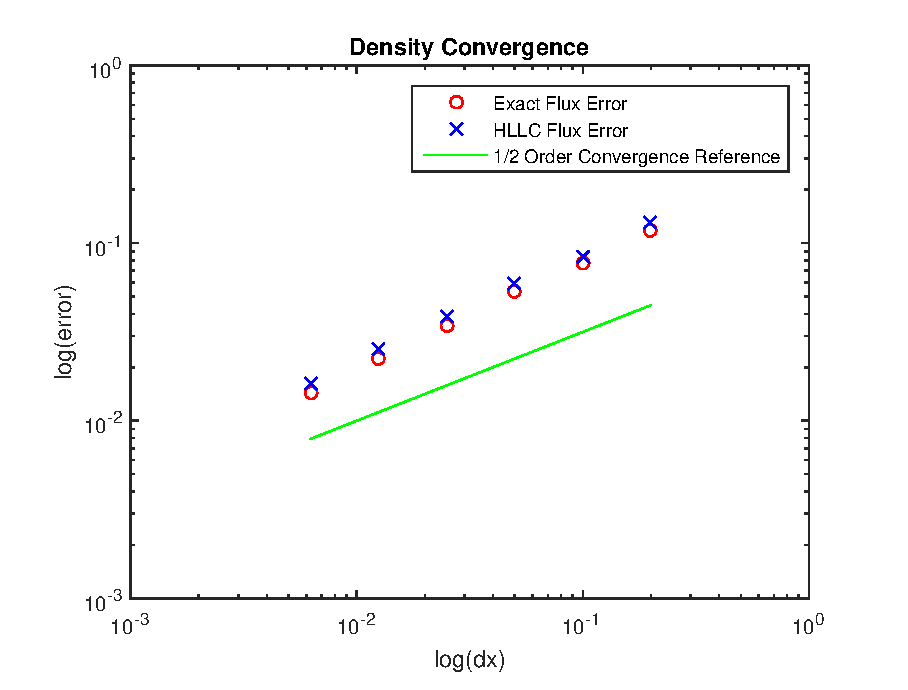
\includegraphics[width=3in]{eulerconv1}
%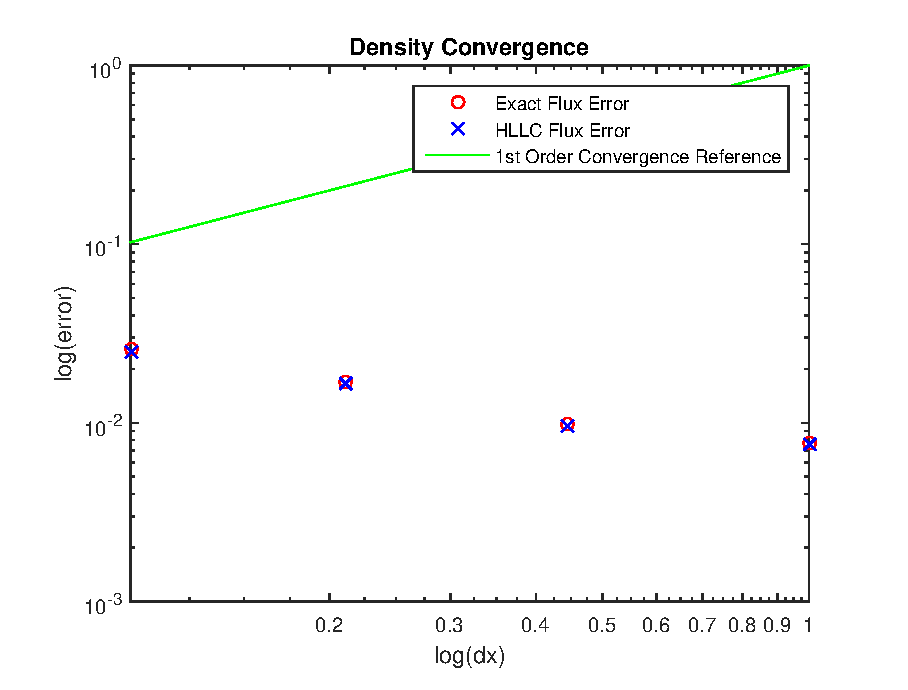
\includegraphics[width=2in]{eulerconv2}
\end{figure}
\end{frame}

\subsection{Simulation Results}
\begin{frame}{Simulation Results}

\end{frame} 



\section{Non-Cartesian Domains}
\begin{frame}{Non-Cartesian Domains}
Smooth, invertible mapping $\mbf{x}=C_g(\mbf{r})$ from parameter space $\mbf{r}=(r,s)$ to physical space $\mbf{x}=(x,y)$
\begin{figure}[h]
\centering
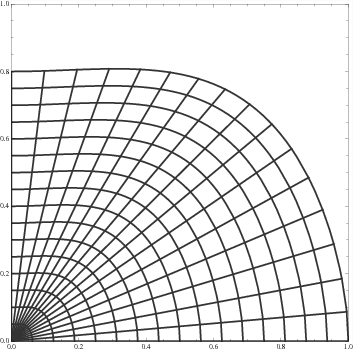
\includegraphics[width=2in]{curvGrid}
\end{figure}
\end{frame}

\subsection{Transformed Equations}
\begin{frame}{Equations in Parameter Space}
The mapping $C_g$ results in the transformed conservation law
\bq \mbf{\phi}_t+\mbf{f}(\mbf{\phi})_r+\mbf{g}(\mbf{\phi})=0,\eq
where
\bq \mbf{\phi}=J \mbf{U},\;\; \mbf{f}=y_s\mbf{F}-x_s\mbf{G},\;\; \mbf{g}=-y_r\mbf{F}+x_r\mbf{G},\eq
and
$$J(r,s)=\left|\frac{\partial(x,y)}{\partial(r,s)}\right|.$$
\end{frame}

\subsection{Numerical Method}
\begin{frame}{Discretization}
Grid: $(r_i,s_j)=(i\Delta r,j\Delta s)$\\
Cell Average: $\mbf{\phi}_{i,j}^n=\frac{1}{\Delta r\Delta s}\int_{s_{j-1}}^{s_j}\int_{r_{i-1}}^{r_i}\mbf{\phi}(r,s,t_n)drds$\\
Conservative Difference Formula:
\bq \mbf{\phi}_{i,j}^{n+1}=\mbf{\phi}_{i,j}^n-\frac{\Delta t}{\Delta r}\left(\mbf{f}_{i,j}^{n+1/2}-\mbf{f}_{i-1,j}^{n+1/2}\right)-\frac{\Delta t}{\Delta s}\left(\mbf{g}_{i,j}^{n+1/2}-\mbf{g}_{i,j-1}^{n+1/2}\right)\eq
Time-Step Restriction Same as in Cartesian Case
\end{frame}

\begin{frame}{Inter-Cell Fluxes}
Godunov - Follow Similar Procedure for Cartesian Domains (Approximate Solver Only)
\bq \begin{split}
&\mbf{\phi}_t+\mbf{f}(\mbf{\phi})_r=0,\;\;\; t>0,\;\; |r|<\infty,\\
&\mbf{\phi}(r,0)=\left\{\begin{array}{cc}\mbf{\phi}_L,&r<0,\\ \mbf{\phi}_R,&r>0\end{array}\right.
\end{split}\eq
Eigenvalue Decomposition of Linearized Jacobian of $\mbf{f}$ Leads to the Numerical Flux
\bq \mbf{f}_{i,j}^{n+1/2}=\left\{\begin{array}{cc}\mbf{f}(\phi_L),&\lambda_1>0,\\
\mbf{f}(\phi_L)+\alpha_1\lambda_1v_1,&\lambda_1<0\text{ and }\lambda_2>0,\\
\mbf{f}(\phi_R)-\alpha_4\lambda_4 v_4,&\lambda_4>0\text{ and }\lambda_2<0,\\
\mbf{f}(\phi_R),&\lambda_4<0.\end{array}\right.\eq
with $\phi_R-\phi_L=\sum_p \alpha_p v_p.$

\end{frame}

\section{Finite Volume - Non-Cartesian Domains}
\subsection{Transformed Equations}
\begin{frame}{Finite Volume - Transformed Equations}
Conservation Equations Satisfied at Discrete Level\\
Cell Average: $\mbf{U}_{j,k}^n=\frac{1}{\Delta x \Delta y}\int_{y_{k-1/2}}^{y_{k+1/2}}\int_{x_{j-1/2}}^{x_{j+1/2}}\mbf{U}(\xi,\eta,t_n)d\xi d\eta$\\
Outward unit vector normal to side $s$ of a grid cell $\mbf{n}_s=(\cos\theta_s,\sin\theta_s)$
Transormed Equation:
\bq \mbf{U}_t=-\frac{1}{|V|}\sum_{s=1}^N\int_{A_s}^{A_{s+1}}[\cos\theta_s\mbf{F}(\mbf{U})+\sin\theta_s\mbf{G}(\mbf{U})]dA\eq
$N=$number of sides of the cell
\end{frame}


\begin{frame}{Transformed Equations}
Rotational Invariance - $\cos\theta_s\mbf{F}(\mbf{U})+\sin\theta_s\mbf{G}(\mbf{U})=\mbf{T}_s^{-1}\mbf{F}(\mbf{T}_s\mbf{U}),$
where $T_s$ is the rotation matrix
$$T_s=\left[\begin{array}{cccc}1&0&0&0\\ 0&\cos\theta&\sin\theta&0\\ 0&-\sin\theta&\cos\theta&0\\ 0&0&0&1\end{array}\right]$$
A Simpler Transformed Equation
\bq \mbf{U}_t=-\frac{1}{|V|}\sum_{s=1}^N\int_{A_s}^{A_{s+1}}\mbf{T}_s^{-1}\mbf{F}(\mbf{T}_s\mbf{U})dA\eq
\end{frame}

\subsection{Numerical Methods}
\begin{frame}{Finite-Volume Numerical Methods}
Intercell Fluxes: $\hat{\mbf{U}}=\mbf{T}_s\mbf{U}$, $\hat{\mbf{F}}=\mbf{F}(\hat{\mbf{U}})$
\bq \begin{split} &\hat{\mbf{U}}_t+\hat{\mbf{F}}_{\hat{x}}=0\\
&\hat{\mbf{U}}(\hat{x},\hat{y},0)=\left\{\begin{array}{cc}\hat{\mbf{U}}_L,&\hat{x}<0\\ \hat{\mbf{U}}_R,&hat{x}>0\end{array}\right.\end{split}\eq
Approximate Integrals in (29)
\bq \int_{A_s}^{A_{s+1}}\mbf{T}_s^{-1}\mbf{F}(\mbf{T}_s\mbf{U})dA\approx L_s\mbf{T}_s^{-1}\hat{\mbf{F}}_s\eq
where $L_s$ is the length of the side $s$.
\end{frame}

\begin{frame}{Discretization}
We now present the final discretization obtained by (30) and (29)
\bq \mbf{U}_{j,k}^{n+1}=\mbf{U}_{j,k}^n-\frac{\Delta t}{|I_{j,k}|}\sum_{s=1}^N L_s\mbf{T}_s^{-1}\hat{\mbf{F}}_s\eq
where $|I_{j,k}|$ is the area of cell $I_{j,k}$. 
Time-Step Restriction is the Same as in the Cartesian Case
\end{frame}

\begin{frame}{Future Steps}
\begin{itemize}
\item Implement and Compare Non-Cartesian Domain Numerical Methods
\item Grid Generation Techniques
\item High-Order Methods (WENO, Slope-correcting/limiting,...)
\item Generalization to 3D Equations
\item ...
\end{itemize}
\end{frame}

\begin{frame}{Sources}
\begin{itemize}
\item Toro, E. F. Riemann Solvers and Numerical Methods for Fluid Dynamics: A Practical Introduction. Berlin: Springer-Verlag, 2009. 
\item Henshaw, William D., and Donald W. Schwendeman. "An Adaptive Numerical Scheme for High-speed Reactive Flow on Overlapping Grids." (2003)
\end{itemize}
\end{frame}

\begin{frame}
Thanks for your time!
\end{frame}


\end{document}